\documentclass[
	noheader
]{coursclass}

\begin{document}

\newcommand{\Propriete}{
	\begin{propriete}[Colinéarité]
		Si $\vec{u}\begin{pmatrix} x \\ y \end{pmatrix}$ et $\vec{v}\begin{pmatrix} x' \\ y' \end{pmatrix}$, alors $\vec{u}$ et $\vec{v}$ sont colinéaires si, de manière équivalente, on a : \medskip
	
		\begin{minipage}{0.7\textwidth}
			\begin{itemize}
				\item \correction{$\vec{u} = k\vec{v}$, avec $k$ un nombre réel ;}
				\item \correction{Les coordonnées de $\vec{u}$ et $\vec{v}$ sont proportionnelles ;}
				\item \correction{$x × y' = x' × y$}
			\end{itemize}
		\end{minipage}
		\begin{minipage}{0.25\textwidth}
			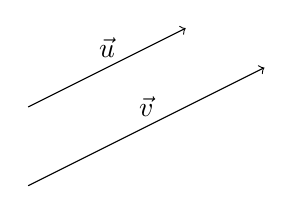
\begin{tikzpicture}
				\draw[->] (0,1) -- node[above] {$\vec{u}$} ++(2,1);
				\draw[->] (0,0) -- node[above] {$\vec{v}$} ++(3,1.5);
			\end{tikzpicture}
		\end{minipage}
	\end{propriete}
}

\Propriete

\vfill

\Propriete

\vfill

\Propriete

\vfill

\Propriete

\vfill

\Propriete

\end{document}